% arara: pdflatex
% arara: bibtex
% arara: pdflatex
% arara: pdflatex
\documentclass[12pt]{article}
\usepackage{amsmath}
\usepackage{graphicx}
\usepackage{hyperref}
\usepackage{textcomp}
\usepackage[section]{placeins}
\usepackage{hhline}
\usepackage{float}
\usepackage{caption} 
\usepackage{enumitem}

\captionsetup[table]{skip=10pt}

\bibliographystyle{acm}

\hypersetup{
  colorlinks, linkcolor=red
}

\begin{document}


\title{CS838 Project Progress Report}
\author{Sek Cheong}
\maketitle

\section{Background}
We proposed a project to use deep CNN to colorize black and white images automatically. We would explore the technique transfer learning to transfer the learned weights from VGG16 to build a new model for colorizing image. We would also compare the result using transfer learning verses training the model from scratch. The report describes the progress we have made so for in our proposed project. We also address the issues we have encountered and the remaining work towards the completion of the project. 


\section{Progress}
We started out by finding the suitable data set for our colorizing model. We then did some research on digital image processing with specific area in color theory and image compression. We defined the model based on the image compress technique we learned to best suited for the task for colorizing.

\subsection{Data Set}
There are a number of data sets for computer vision available publicly. Among the available image data sets the ImageNet data set is the most famous one. Many machine learning models involving vision are trained on ImageNet images. There are approximately one million image files from $1000$ categories in the ImageNet data set and about $120$G in size. We downloaded (took really long time!) the entire image set and looked some images. It turned that there are many images either in black and white or were not useful coloring examples. We believe a good coloring example image should contain a single object, the foreground and background should be distinguishable and should have good saturation and hue. It would be impossible to hand pick the good examples given the time constrain and the shear number of images in the data set. For this reason we switched to MIRFLICKR~\cite{MIR08} which is a collection of images from the flicker picture sharing website. The MIRFLICKR pictures are very appearing visually because a lot of them were produced by photographer users from flicker. 

We picked the first $10000$ images (black and white images were excluded) from MIRFLICKR as our image set. The images was then split into $70\%$ for training, $20\%$ for tuning, and the remaining $10\%$ for testing. 

\begin{figure}[!ht]
 \centering
  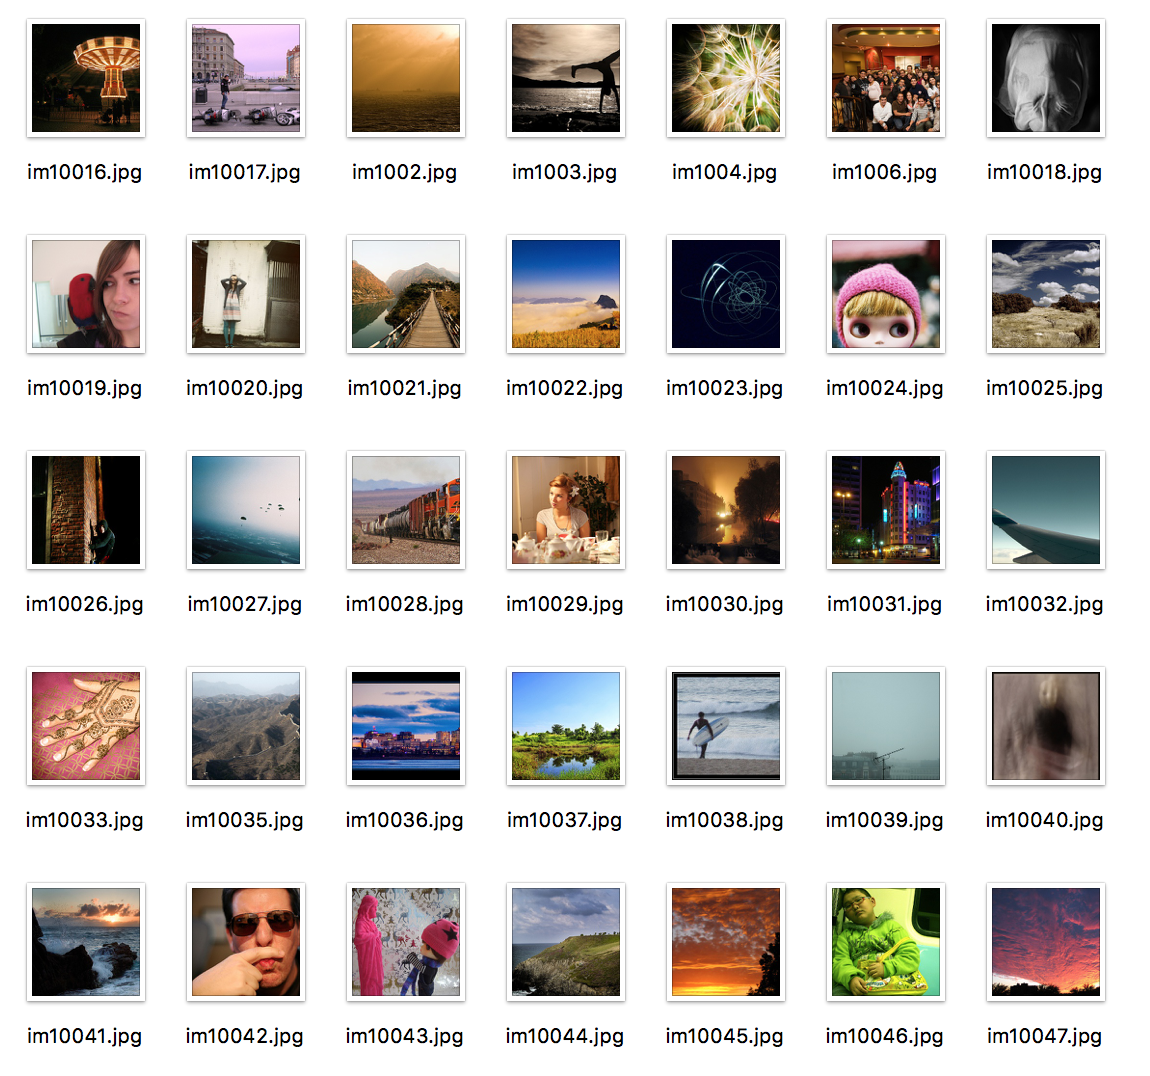
\includegraphics[width=4.0in]{resource/exampleimages.png}
 \label{sampleimages}
 \caption{Some sample images from our training set}
\end{figure}


The images were come in various sizes but for out model we use accepts images of $224\times224$ pixels. The rational for choosing such image size was because the images trained on VGG16 were $224\times224$ pixels and we would use VGG16 weights for training our own model. To make the MIRFLICKR images compatible with our model we need to resize the images into $224\times224$ pixels. However, instead of simply resizing the images into $224\times224$ pixels, we scale the shorter side of the image to $224$ pixels and crop the image along with the $224$ pixel side to  $224\times224$ pixels. We think training on images with the correct aspect ration might give a better result for coloring. The scaling and cropping was done by a python script~\cite{PYDATA} we created.

To construct a training example from a color image we could convert the image into gray scale image and use the gray scale image as input $\boldsymbol{X}$, and the RGB values as the target $\boldsymbol{Y}$. Note, the input is a $1\times224\times224$ vector and the target is a $3\times224\times224$ vector. As explained by Ryan Dahl\textquotesingle s web blog post~\cite{RYAN2016} that we could convert the image from RGB color space into YUV color space, where Y is the intensity of the image, and UV are two chrominance components of the image. This reduces the target vector $\boldsymbol{Y}$ to $2\times224\times224$. The following figure shows the original image, the Y component, the U component, and the V component. 

\begin{figure}[!ht]
 \centering
  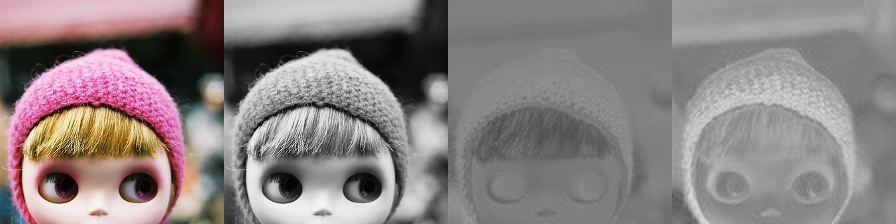
\includegraphics[width=5.0in]{resource/YUV.png}
 \label{yuvimage}
 \caption{The original picture and its YUV components}
\end{figure}


\subsection{Model}
We use the VGG16 model as our starting model as shown in Figure 3. The VGG16 has an output layer of $1000$ units with Softmax activation. The output layer is designed in such a way that it can be used to classify image from a thousand categories. Our initial design of transfer learning was that after loading the weights for the model we remove the final layer and replace with a $2\times224\times224$ regression unit. For activation function we use the hyperbolic tangent function. This proved to be a disaster as the number of parameters in the model skyrocketed to $545,402,688$! from  $138,357,544$. 


\begin{figure}[H]
 \centering
  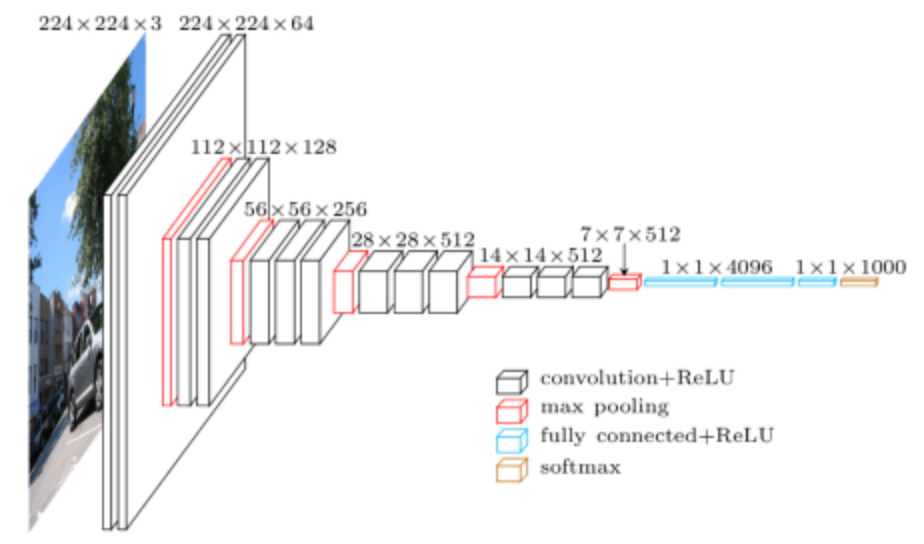
\includegraphics[width=5.0in]{resource/vgg16.png}
\center
\label{fig:vggvis}
 \caption{The VGG16 model visualization}
\end{figure}

It turns out that YUV color space is closely related YCbCr color space which was used for digital encoding of color information suited for video and still-image compression and transmission such as MPEG and JPEG~\cite{YUVWIKI}. For our use we could simply treat UV as same as CbCr. The main difference between these two color spaces was scaling. Since we scale pixel values between $-1$ and $1$, it wouldn't make any difference for us. The nice property of YCbCr color space was that human eyes are far more sensitive to change in intensity than color. This allowed us to throw away most of the CbCr information while still maintain the image quality. The process of throwing away color information is called color space compression. 

We experimented around different compression rate and it appeared that we can throw away $80\%$ of the color information and the image still maintains very good color quality. 


\begin{figure}[H]
 \centering
  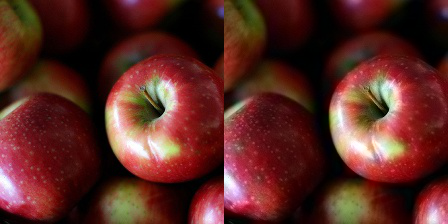
\includegraphics[width=5.0in]{resource/colorcompress.png}
 \label{yuvimage}
 \caption{Image on the left with $90\%$ color space compression}
\end{figure}

As show in the figure above, the image on the left is the original image, the image on the right has $90\%$ of the color information removed.


\begin{table}[H]
	\caption{The colorize model (with color space compression) based on VGG16 architecture}
  	\centering
	\begin{tabular}{|l|l|r|}
		\hline 
		Layer (type)                  &  Output Shape           &    Parameters  \\ \hhline{|=|=|=|}
		input 1 (Input Layer)         &  (None, 224, 224, 3)    &    0           \\ \hline
		block 1 conv 1 (Conv 2D)      &  (None, 224, 224, 64)   &    1792        \\ \hline 
		block 1 conv 2 (Conv 2D)      &  (None, 224, 224, 64)   &    36928       \\ \hline 
		block 1 pool (Max Pooling 2D) &  (None, 112, 112, 64)   &    0           \\ \hline 
		block 2 conv 1 (Conv 2D)      &  (None, 112, 112, 128)  &    73856       \\ \hline 
		block 2 conv 2 (Conv 2D)      &  (None, 112, 112, 128)  &    147584      \\ \hline 
		block 2 pool (Max Pooling 2D) &  (None, 56, 56, 128)    &    0           \\ \hline 
		block 3 conv 1 (Conv 2D)      &  (None, 56, 56, 256)    &    295168      \\ \hline 
		block 3 conv 2 (Conv 2D)      &  (None, 56, 56, 256)    &    590080      \\ \hline 
		block 3 conv 3 (Conv 2D)      &  (None, 56, 56, 256)    &    590080      \\ \hline 
		block 3 pool (Max Pooling 2D) &  (None, 28, 28, 256)    &    0           \\ \hline 
		block 4 conv 1 (Conv 2D)      &  (None, 28, 28, 512)    &    1180160     \\ \hline 
		block 4 conv 2 (Conv 2D)      &  (None, 28, 28, 512)    &    2359808     \\ \hline 
		block 4 conv 3 (Conv 2D)      &  (None, 28, 28, 512)    &    2359808     \\ \hline 
		block 4 pool (Max Pooling 2D) &  (None, 14, 14, 512)    &    0           \\ \hline 
		block 5 conv 1 (Conv 2D)      &  (None, 14, 14, 512)    &    2359808     \\ \hline 	
		block 5 conv 2 (Conv 2D)      &  (None, 14, 14, 512)    &    2359808     \\ \hline 
		block 5 conv 3 (Conv 2D)      &  (None, 14, 14, 512)    &    2359808     \\ \hline 
		block 5 pool (Max Pooling 2D) &  (None, 7, 7, 512)      &    0           \\ \hline 
		flatten (Flatten)             &  (None, 25088)          &    0           \\ \hline 
		fc 1 (Dense)                  &  (None, 4096)           &    102764544   \\ \hline 
		fc 2 (Dense)                  &  (None, 4096)           &    16781312    \\ \hline 
		colorize (Dense)              & (None, 2178)            &    8923266     \\ \hline 
	\end{tabular}
\end{table}


We discarded $85\%$ of the color information, that is we resize the chrominance components UV to $15\%$ of its original size using bi-cubic interpolation. This process reduced the UV size down to $33\times33$ from $224\times224$. We adjusted the output layer to the size of reduced color dimension and the parameters went from $545{,}402{,}688$ to $143{,}183{,}810$. 


\subsection{Training}
We trained out model on $1500$ images with $50$ epoch, the training set is hardly large enough to train a complex task such as colorization, but due to the limited computing resources (more on that in the Challenges section) and time constrain, we had to settle with $1500$ samples. The training process took about $25$ hours to complete. We hadn't really had a chance to try different hyper-parameters, optimizers, and loss functions. We simply configured our model to use GSD and MSE. 



\begin{figure}[H]
 \centering
  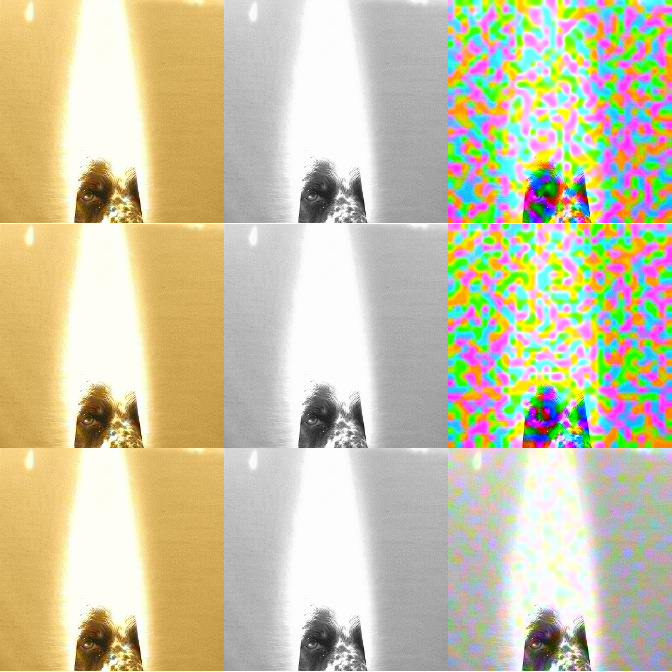
\includegraphics[width=5.0in]{resource/trainstage.png}
 \label{yuvimage}
 \caption{Predictions in various epoch, left the ground truth, middle the input image, right the predicted image}
\end{figure}


Here are some predicted images:

\begin{figure}[H]
 \centering
 \includegraphics[width=5.0in]{resource/im25.jpg}
\end{figure}


\begin{figure}[H]
 \centering
 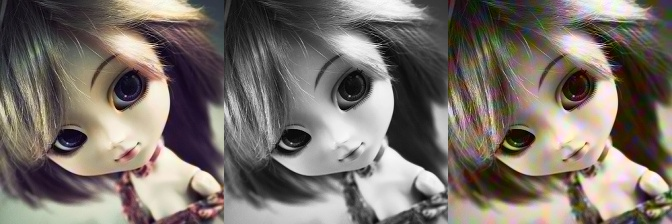
\includegraphics[width=5.0in]{resource/im43.jpg}
\end{figure}



\begin{figure}[H]
 \centering
 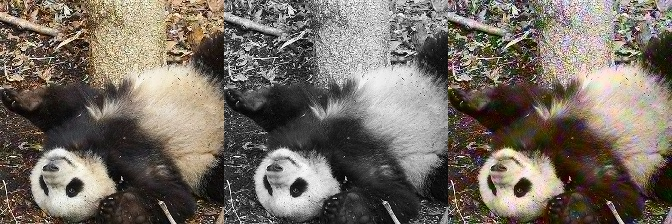
\includegraphics[width=5.0in]{resource/im89.jpg}
\end{figure}


\begin{figure}[H]
 \centering
 \includegraphics[width=5.0in]{resource/im94.jpg}
\end{figure}


\section{Challenges}
One of the major challenges were getting the various pieces of software to work on our MacPro workstation machine. We used OpenCV for image manipulations however OpenCV did not have bindings for Python3 and we had to build it from source and it was not an easy task due to various dependent components we also had to build. 

For tensorflow the default version installed via pip was not optimized to use vector instructions (such as SSE, AVX) on Intel processors. After much research on the Internet we were able to build the tensorflow from source. Getting tensorflow to work with GPU (Nvidia CUDA library, don't even try OpenCl!) was another challenge in that the CUDA library is very fussy on the versions of LLVM compiler on OSX. We had to downgrade the LLVM compiler on our Mac to a lower version in order to compile with the CUDA library. 

The major shock came as we try to train our model on GPU enabled tensorflow we discovered that our GPU, nVidia GeForce GTX 660, only supports CUDA compute capability 3.0 whatever that is, but the minimum requirement for tensorflow is 3.5. We were not be able to run every planned experiments. 


\section{Remaining Tasks}
So far we were only able to train 1500 samples with 50 epochs. Each epoch took about half hour to complete. Ideally we would like to train at lease 7000 examples, but due to the GPU failure and the given time constrain, we were not able to perform such tarining. With that said we would like to do the following:

\begin{enumerate}[label=(\roman*)]
\item Modify our loss function to better optimize colorization. It might be worth while to try a Euclidean distance between the true and predicted color components: $\sqrt{(U-\hat{U})^2+(V-\hat{V})^2}$
\item Plot the model accuracy and model loss curve
\item Try some different optimization such as Adam update, batch normalization, etc. 
\item If time permits create visualization of weights in various layers~\cite{VISW}.
\end{enumerate}


\bibliography{biblio}

\end{document}